\documentclass[12pt, titlepage]{article}

\usepackage{booktabs}
\usepackage{tabularx}
\usepackage{hyperref}
\hypersetup{
    colorlinks,
    citecolor=black,
    filecolor=black,
    linkcolor=red,
    urlcolor=blue
}
\usepackage[round]{natbib}

\title{SE 3XA3: Software Requirements Specification\\PasswordProtectionProgram}

\author{Team 28, Tuples1
		\\ Shabana Dhayananth dhayanas
		\\  Suhavi Sandhu sandhs11
		\\ Joseph Lu luy89
}

\date{\today}

\begin{document}

\maketitle

\pagenumbering{roman}
\tableofcontents
\listoftables
\listoffigures

\begin{table}[bp]
\caption{\bf Revision History}
\begin{tabularx}{\textwidth}{p{3cm}p{2cm}X}
\toprule {\bf Date} & {\bf Version} & {\bf Notes}\\
\midrule
Date 1 & 1.0 & Notes\\
Date 2 & 1.1 & Notes\\
\bottomrule
\end{tabularx}
\end{table}

\newpage

\pagenumbering{arabic}

This document describes the requirements for ....  The template for the Software
Requirements Specification (SRS) is a subset of the Volere
template~\citep{RobertsonAndRobertson2012}.  If you make further modifications
to the template, you should explicity state what modifications were made.

\section{Project Drivers}

\subsection{The Purpose of the Project}

The purpose of this project is to implement an encrypted password manager,  PasswordProtectionProgram (PPP) 
wherein a person can safely store and access all of the passwords they use with a single master password. 
Through working on this project the software team also hopes to learn about encryption methods and the 
development process.

\subsection{The Stakeholders}

The stakeholders of this project are:
\begin{itemize}
\item Users of online services that want a place to store their passwords safely and generate stronger passwords
\item Services for which the passwords are created as they have to deal with security threats and users that forget their passwords
\item Identity thieves since they are able to breach users’ personal information due to weak passwords and weak encryption methods
\item The development team, as they are the students attempting to solve the problem at hand
\end{itemize}

\subsubsection{The Client}

\subsubsection{The Customers}

\subsubsection{Other Stakeholders}

\subsection{Mandated Constraints}

\subsubsection{Solution Constraints}

\textbf{Description}: The product shall operate on all Operating Systems with python installed. (i.e. Windows, OSX, Linux) through a gui app.
\\
\textbf{Rationale}: The client will use all of these operating systems
\\
\textbf{Fit criterion}: The product shall be approved by testing groups of each operating system.

\subsubsection{Partner or Collaborative Applications}

The product does not have any direct partner or collaborative applications. This product is fully built on python and MariaDB and will be able to be executed in the desktop.

\subsubsection{Off-the-Shelf Software}

The off-the-shelf software required for this product to be implemented:
\begin{itemize}
\item Python
\item MariaDB
\item Tkinter (python library)
\end{itemize}
All the software that is required is open source and can be found on the internet.

\subsubsection{Budgeting Constraints}

The budget of our project is zero dollars so no further purchases are required.

\subsubsection{Schedule Constraints}

There is a deadline in December for the project to be completed.

\subsubsection{Naming Conventions and Terminology}

\subsection{Naming Conventions and Terminology}

\subsection{Relevant Facts and Assumptions}

Some relevant facts regarding this project are that the original program has 29850 lines of code. 
The program has a GNU General Public Licence v3.0 licence and can be run on Windows, Unix and Linux 
operating systems as well as iOS and Android mobile devices. The team will be using symmetric encryption
 from the cryptography library, which implements AES with a 128-bit key for encryption. AES is chosen by the 
U.S. government to protect classified information throughout the world to encrypt sensitive data. A relevant 
fact about passwords that has to do with the project is that passwords are easily hacked because humans 
follow similar patterns. For instance, the numbers ‘1’ and ‘2’ are common and capital letters are often used at
 the beginning of passwords. Lastly, it should be noted that the original product implemented AES and used 
PBKDF2, a key derivation function that reduces the chance of brute force attacks.
\\
\\
Some assumptions made the developers are that the cryptography library will be enough for our needs and does
 not need to be tested for its encryption since that would require executing brute force attacks. Also, it is 
assumed that there is a need for users to store their usernames and passwords safely. Lastly, it is assumed 
that Python code can run on Windows, Unix and Linux environments. 

\section{Functional Requirements}

\subsection{The Scope of the Work and the Product}

We will be re-implementing the original open source software (Padlock) as an offline, 
desktop application, suitable for Windows, Macintosh or Unix environments. This is due to time 
constraints set by the project deadline as well as further security by not having the product online. 
Also, the Python cryptography library will be used for the encryption as the development team does not 
have experience creating secure encryption methods. 

\subsubsection{The Context of the Work}

Almost all services provided to consumers, including banking, health records and social media, 
stores sensitive personal information in a password protected account. However, strong passwords are 
often easy to forget and therefore, people usually opt for weaker passwords or use the same 
one for multiple accounts. This makes them more susceptible to security threats.

\subsubsection{Work Partitioning}

\subsubsection{Individual Product Use Cases}

\begin{figure}[h]
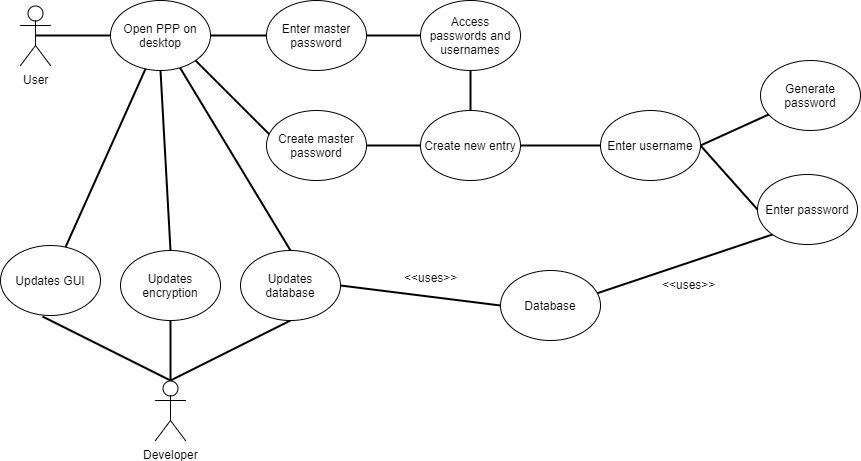
\includegraphics{Images/UseCase.png}
\caption{Figure 1: Use Case Diagram}
\end{figure}

\begin{figure}[h]
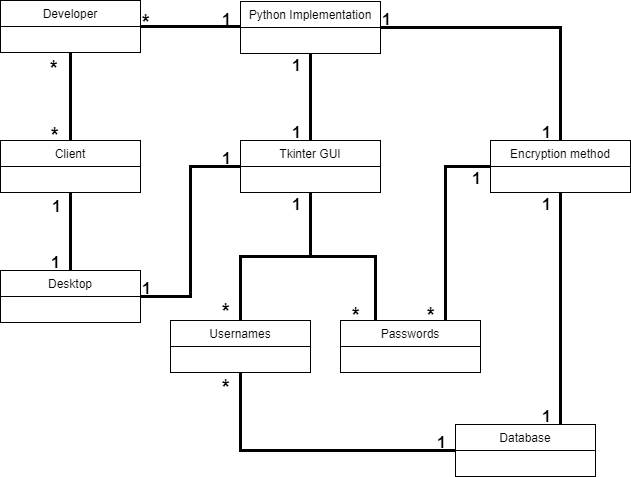
\includegraphics{Images/BusinessModel.png}
\caption{Figure 2: Business Data Model}
\end{figure}

\subsection{Functional Requirements}

\begin{center}
\begin{tabular}{ | p{1cm} | p{4cm} | p{4cm} | p{4cm} | }
	\hline
	Name & Description & Rationale & Fit Criterion\\
	\hline
	FR1 & The executaable Python code will create a user interface window & To allow user to use the application & Run application \\
	\hline
	FR2 & Upon execution, the program will have a connection to a local database & To allow the program to store usernames and encrypted passwords & Create a new entry and check if it shows up on DB \\
	\hline
	FR3 & The user must be able to create a master password & To ensure that only the user can access the data & When opening the app for the first time, create master password and use it \\
	\hline
	FR4 & The user must be able to enter a master password & To access and create passwords and usernames & Enter correct PW and incorrect PW \\
	\hline
	FR5 & The new user must be able to add a new entry & To allow the user to store a new username and password & Create new entry, close app and verify it exists in DB \\
	\hline
	FR6 & The user should be able to generate a random password & To allow for a stronger password & Generate multiple PWs and verify randomness \\
	\hline
	FR7 & The user interface must have a link to the user manual & To aid the user in using the software & Manual link should take user to manual \\
	\hline
	FR8 & After one minute of inactivity, the application should go to the home screen & To protect the users’ data & Keep app running for 1 minute \\
	\hline
	FR9 & The application should have buttons to directly copy username and password & To allow user to easily input long usernames or passwords & Copy existing password and verify that it pastes onto various text inputters \\
	\hline
	FR10 & The user should be able to change their master password & To allow the user to regularly update PW & Update PW from Settings and verify that new PW works and old one does not \\
\hline
\end{tabular}
\end{center}

\section{Non-functional Requirements}

\subsection{Look and Feel Requirements}

\subsection{Usability and Humanity Requirements}

\subsection{Performance Requirements}

\subsection{Operational and Environmental Requirements}

\subsection{Maintainability and Support Requirements}

\subsection{Security Requirements}

\subsection{Cultural Requirements}

\subsection{Legal Requirements}

\subsection{Health and Safety Requirements}

This section is not in the original Volere template, but health and safety are
issues that should be considered for every engineering project.

\section{Project Issues}

\subsection{Open Issues}

Actions to be taken in the cases in which the user has lost access to their passwords or has lost all of their information due to hardware problems have not yet been explored. Also, the product will be implemented on a Windows operating system as that is the operating system used by all team members. It is intended that the software will work on Linux and Unix operating systems as well so but testing on those environments has not been discussed.

\subsection{Off-the-Shelf Solutions}

\subsection{New Problems}

If users solely on this product to store all of their passwords, there is potential for them to lose all of their saved data due to a hashing issue, hardware issue or in the theft or loss of their computer. The product requires that the user to enter their current master password in order to change it which could cause issues in the case that they forget it.

\subsection{Tasks}

Deliverables as outlined by SFWRENG 3XA3 courseware:

table

Implementation Breakdown:

other table

The team will be implementing and testing non-functional requirements based on their priority.

\subsection{Migration to the New Product}

The final product will be run and installed via an executable Python file. As MariaDB will be used to store the usernames and passwords, the database will have to be converted before the product is released. It also needs to be tested on all intended operating systems.

\subsection{Risks}

Security is the main concern for this project as the team is not explicitly testing the strength of the encryption method under the assumption that the cryptography library is reliable. The probability of this becoming a problem is unlikely as the product will be offline and will not be a target of many attacks. If the problem does occur, the team will look into a more complex encryption method. 

\subsection{Costs}

Not applicable in the case that all required dependencies are open-source or free.

\subsection{User Documentation and Training}

There will be a concise and useful manual that provides instructions on how to use the product. To make the product easier to use, the team will be testing for the GUI’s user-friendliness and receiving feedback from others. 

\subsection{Waiting Room}

Ideally, there would be a backup data option for the user to use as a precaution in the case of hardware 
failure and loss of data.
\\
To improve the user interface, it would be nice to provide support for multiple languages (other than only English).
\\
Passwords can be organized by service in the database, so based on that there can be different levels of security provided. For example, bank passwords and library account passwords don’t need the same level of security.

\subsection{Ideas for Solutions}

Instead of storing passwords, another solution is 2 factor authentication (2FA). This eliminates the need to download a password management software and instead the user can do a phone verification after typing their password or a fingerprint scanner for mobile devices.

\begin{figure}[h]
\includegraphics{Images/2fa.png}
\caption{Figure 3: 2 Factor Authentication}
\end{figure}

\bibliographystyle{plainnat}

\bibliography{SRS}

\newpage

\section{Appendix}

This section has been added to the Volere template.  This is where you can place
additional information.

\subsection{Symbolic Parameters}

The definition of the requirements will likely call for SYMBOLIC\_CONSTANTS.
Their values are defined in this section for easy maintenance.


\end{document}
